\section{\PostNet}
\label{sec:model_006}

In classification, we can distinguish between two types of uncertainty for a given input $\vect{x}\dataix$: the uncertainty on the class prediction \smash{$y\dataix \in \{1, \ldots, \nclass\}$} (i.e.\ aleatoric unceratinty), and the uncertainty on the categorical distribution prediction \smash{$\vect{p}\dataix = [p\dataix_1, \ldots, p\dataix_\nclass]$} (i.e.\ epistemic uncertainty). A convenient way to model both is to describe the \emph{epistemic distribution} \smash{$q\dataix$} of the categorical distribution prediction \smash{$\vect{p}\dataix$}, i.e.\ \smash{$\vect{p}\dataix \sim q\dataix$}. From the epistemic distribution follows naturally an estimate of the \emph{aleatoric distribution} of the class prediction \smash{$y\dataix \sim \text{Cat}(\bar{\vect{p}}\dataix)$} where \smash{$\E_{q\dataix}[\vect{p}\dataix] = \bar{\vect{p}}\dataix$}.

Approaches like ensembles \cite{ensembles} and dropout \cite{dropout} model $q\dataix$ implicitly, which only allows them to estimate statistics at the cost of $S$ samples (e.g. \smash{$\E_{q\dataix}[\vect{p}\dataix] \approx \frac{1}{S}\sum_{s=1}^{S} \tilde{\vect{p}}\dataix$} where \smash{$\tilde{\vect{p}}\dataix$} is sampled from \smash{$q\dataix$}). 
%
Another class of models \cite{PriorNetworks, reverse-kl, uceloss, sensoy2018} explicitly parametrizes the epistemic distribution with a Dirichlet distribution (i.e.\ \smash{$q^{(\idata)} = \text{Dir}(\bm{\alpha}\dataix)$} where \smash{$f_{\theta}(x\dataix) = \bm{\alpha} \dataix \in \mathbb{R}_+^\nclass$}), which is the natural prior for categorical distributions. This parametrization is convenient since it requires only one pass to compute epistemic distribution, aleatoric distribution and class prediction:
\begin{equation}
\begin{aligned}
q^{(\idata)} &= \text{Dir}(\bm{\alpha}\dataix),\hspace{25pt} 
\bar{p}_\iclass\dataix &= \frac{\alpha_\iclass}{\alpha_0} \text{ with } \alpha_0 = \sum^{\nclass}_{\iclass=1} \alpha_\iclass,\hspace{25pt}
y^{(\idata)} &= \arg \max \;[\bar{p}_1, ..., \bar{p}_\nclass]
\end{aligned}
\end{equation}
The concentration parameters \smash{$\alpha\dataix_\iclass$} can be interpreted as the number of observed samples of class $\iclass$ and, thus, are a good indicator of epistemic uncertainty for non-degenerate Dirichlet distributions (i.e.\ \smash{$\alpha\dataix_\iclass \geq 1$}). To learn these parameters, Prior Networks \cite{PriorNetworks, reverse-kl} use OOD samples for training and define different target values for ID and OOD data. For ID data, \smash{$\alpha\dataix_\iclass$} is set to an arbitrary, large number if $\iclass$ is the correct class and $1$ otherwise. For OOD data, \smash{$\alpha\dataix_\iclass$} is set to $1$ for all classes. 

This approach has four issues:
%\begin{itemize}
    %\item 
    \textbf{(1)} The knowledge of OOD data for training is unrealistic. In practice, we might not have these data, since OOD samples are by definition not likely to be observed.
    %\item 
    \textbf{(2)} Discriminating in- from out-of-distribution data by providing an explicit set of OOD samples is hopeless. Since any data not from the data distribution is OOD, it is therefore impossible to characterize the infinitely large OOD distribution with an explicit data set.
    %\item 
    \textbf{(3)} The predicted Dirichlet parameters can take any value, especially for new OOD samples which were not seen during training. In the same way, the sum of the total fictitious prior observations over the full input domain $\int \alpha_0(\vect{x}) d\vect{x}$  is not bounded and in particular can be much larger than the number of ground-truth observations $N$. This can result in undesired behavior and assign arbitrarily high epistemic certainty for OOD data not seen during training.
    %\item 
    \textbf{(4)} Besides producing such arbitrarily high prior confidence, PNs can also produce degenerate concentration parameters (i.e.\ $\alpha_\iclass$ < 1). While \cite{reverse-kl} tried to fix this issue by using a different loss, nothing intrinsically prevents Prior Networks from predicting degenerate prior distributions.
%\end{itemize}
In the following section we describe how \PostNet solves these drawbacks.

\subsection{An input-dependent Bayesian posterior}

First, recall the Bayesian update of a single categorical distribution \smash{$y \sim \text{Cat}(\vect{p})$}. It consists in (1) introducing a prior Dirichlet distribution over its parameters i.e. $\prob(\vect{p}) = \text{Dir}(\bm{\beta^\text{prior}})$ where \smash{$\bm{\beta^\text{prior}} \in \mathbb{R}_+^\nclass$}, and (2) using $N$ given observations \smash{$y^{(1)},..., y^{(N)}$} to form the posterior distribution $\prob(\vect{p}|\{y^{(j)}\}_{j =1}^N)= \text{Dir}(\bm{\beta^\text{prior}} + \bm{\beta^\text{data}})$ where \smash{$\beta^\text{data}_\iclass = \sum_j \mathbbm{1}_{y^{(j)}=\iclass}$} are the class counts. That is, the Bayesian update is
\begin{equation}
    \begin{aligned}
    \prob(\vect{p}|\{y^{(j)}\}_{j =1}^n) \propto \prob(\{y^{(j)}\}_{j =1}^n|\vect{p}) \times \prob(\vect{p}).
    \end{aligned}
\end{equation}
Observing no data (i.e. $\beta_\iclass^\text{data} \rightarrow 0$) would lead to flat categorical distribution (i.e. \smash{$p_\iclass = {\beta_\iclass^{\text{prior}}}\cdot ({\sum_{\iclass'}\beta_{\iclass'}^{\text{prior}}})^{-1}$}), while observing many samples (i.e. \smash{$\beta_\iclass^\text{data}$} is large) would converge to the true data distribution (i.e. $p_\iclass \approx \frac{\beta_\iclass}{\sum_i\beta_i}$).
Furthermore, we remark that $N$ behaves like a certainty budget distributed over all classes i.e. \smash{$N = \sum_\iclass \beta^\text{data}_\iclass$}.

Classification is more complex. Generally, we predict the class label \smash{$y\dataix$} from a different categorical distribution \smash{$\text{Cat}(\vect{p}\dataix)$} for each input \smash{$\vect{x}\dataix$}. \PostNetacro extends the Bayesian treatment of a single categorical distribution to classification by predicting an individual posterior update for any possible input. To this end, it distinguishes between a fixed prior parameter \smash{$ \bm{\beta}^{\text{prior}}$} and the additional learned (pseudo) counts \smash{$\bm{\beta}\dataix$} to form the parameters of the posterior Dirichlet distribution \smash{$\bm{\alpha}\dataix = \bm{\beta}^{\text{prior}} + \bm{\beta}\dataix$}. 
%\bc{Remark that directly using the single label \smash{$y\dataix$} to learn independently the posterior for input \smash{$\vect{x}\dataix$ (i.e. $\beta_\iclass\dataix = 1$} for the true class and \smash{$\beta_\iclass\dataix = 0$} otherwise) would lead to a poor uncertainty estimate and more importantly not generalize to new inputs}. 
Hence, \PostNetacro's posterior update is equivalent to predicting a set of pseudo observations \smash{$\{\tilde{y}^{(j)}\}_j\dataix$} per input \smash{$\vect{x}\dataix$}, accordingly \smash{$\beta_\iclass\dataix = \sum_j  \mathbbm{1}_{\tilde{y}^{(j)}=\iclass}$} and
\begin{equation}
    \begin{aligned}
    \prob(\vect{p}\dataix|\{\tilde{y}^{(j)}\}_j\dataix) \propto \prob(\{\tilde{y}^{(j)}\}_j\dataix|\vect{p}\dataix) \times \prob(\vect{p}\dataix).
    \end{aligned}
\end{equation}
In practice, we set \smash{$\bm{\beta}^{\text{prior}}=\vect{1}$} leading to a flat equiprobable prior when the model brings no additional evidence, i.e.\ when \smash{$\bm{\beta}\dataix = \vect{0}$}. 

The parametrization of $\beta_\iclass\dataix$ is crucial and based on two main components. The first component is an encoder neural network, $f_{\theta}$ that maps a data point $\vect{x}\dataix$ onto a low-dimensional latent vector $\latent\dataix=f_{\theta}(\vect{x}\dataix) \in \mathbb{R}^{\latentdim}$. The second component is to learn a \textit{normalized} probability density $\prob(\latent | \iclass; \phi)$ per class on this latent space; intuitively acting as class conditionals in the latent space. Given these and the number of ground-truth observations $N_\iclass$ in class  $\iclass$, we define:
\begin{equation}
\begin{aligned}
\label{eq:additional_observations}
	\beta_\iclass\dataix &= N_\iclass \cdot \prob(\latent\dataix | c; \phi) = N \cdot \prob(\latent\dataix | \iclass; \phi) \cdot \prob(\iclass),
\end{aligned}
\end{equation}
which corresponds to the number of (pseudo) observations of class $\iclass$ at $\latent \dataix$. Note that it is crucial that $\prob(\latent | \iclass; \phi)$ corresponds to a proper normalized density function since this will ensure the model's epistemic uncertainty to increase outside the known distribution. Indeed, the core idea of our approach is to parameterize these distributions by a flexible, yet tractable family: normalizing flows (e.g. radial flow \cite{radialflow} or IAF \cite{iaf_flow}). Note that normalizing flows are theoretically capable of modeling any continuous distribution given an expressive and deep enough model \cite{neural_flow, iaf_flow}.

In practice, we observed that various architectures can be used for the encoder. Also, similarly to GAN training \cite{GAN_batch_norm}, we observed that adding a batch normalization after the encoder made the training more stable. It facilitates the match between the latent positions output by the encoder and non-zero density regions learned by the normalizing flows. Remark that we can theoretically use any density estimator on the latent space. We experimentally compared Mixtures of Gaussians (MoG), radial flow \cite{radialflow} and IAF \cite{iaf_flow}. While all density types performed reasonably well (see \cref{fig:unc_sensorless_drive} and app.), we observed a better performance of flow-based density estimation in general. We decided to use radial flow for its good trade-off between flexibility, stability, and compactness (only few parameters).

\paragraph{Model discussion.} The \cref{eq:additional_observations} exhibits a set of interesting properties which ensure reasonable uncertainty estimates for ID and OOD samples. To highlight the properties of the Dirichlet distributions learned by \PostNetacro, we assume in this paragraph that we have a fixed encoder $f_\theta$ and normalizing flow model parameterized by $\phi$. Writing the mean of the Dirichlet distribution parametrized by \cref{eq:additional_observations} and using Bayes' theorem gives:
\begin{equation}
\E_{\vect{p}\sim \Dir(\mathbf{\alpha}\dataix)}[p_\iclass] = \frac{\beta_\iclass^\text{prior} + N \cdot \prob(\iclass | \latent\dataix; \phi) \cdot \prob(\latent\dataix; \phi)}{\sum_\iclass\beta_\iclass^\text{prior} + N \cdot \prob(\latent\dataix; \phi)}
\end{equation}
For very likely in-distribution data (i.e. $\prob(\latent\dataix ; \phi) \rightarrow \infty$), the aleatoric distribution estimate \smash{$\bar{\vect{p}}\dataix = \E_{\vect{p}\sim \Dir(\mathbf{\alpha}\dataix)}[p_\iclass]$} converges to the true categorical distribution \smash{$\prob(\iclass|\latent \dataix; \phi)$}. Thus, predictions are more accurate and calibrated for likely samples. Conversely, for out-of-distribution samples (i.e. \smash{$\prob(\latent\dataix ; \phi) \rightarrow 0$}), the aleatoric distribution estimate \smash{$\bar{\vect{p}}\dataix = \E_{\vect{p}\sim \Dir(\mathbf{\alpha}\dataix)}[p_\iclass]$} converges to the flat prior distribution (e.g. \smash{$p_\iclass=\frac{1}{\nclass}$} if \smash{$\bm{\beta}^{prior}=\vect{1}$}). In the same way, we show in the appendix that the covariance of the epistemic distribution converges to $\vect{0}$ for very likely in-distribution data, meaning no epistemic uncertainty. Thus, uncertainty for in-distribution data is reduced to the (inherent) aleatoric uncertainty and zero epistemic uncertainty.
%
Similarly to the single categorical distribution case, increasing the training dataset size (i.e. $N \rightarrow \infty$) also leads to the mean prediction $\E_{\vect{p}\sim \Dir(\mathbf{\alpha})}[p_\iclass]$ converging to the class posterior \smash{$\prob(c | \latent\dataix; \phi)$}. On the contrary, no observed data (i.e $N=0$) again leads to the model reverting to a flat prior.

\PostNet also handles limited certainty budgets at different levels. At the sample level, the certainty budget \smash{$\alpha_0\dataix = \sum_\iclass \alpha_\iclass\dataix$} is distributed over classes. At the class level, the certainty budget \smash{$N_\iclass = \int N_\iclass \; \prob(\latent | c; \phi) \; d\latent = N_\iclass  \int \prob(\latent | c; \phi) \; d\latent$} is distributed over samples. At the dataset level, the certainty budget \smash{$N = \sum_\iclass \int N_\iclass \; \prob(\latent | c; \phi) \; d\latent$} is distributed over classes and samples. Regions of latent space with many training examples are assigned high density $\prob(\latent | c; \phi)$, forcing low density elsewhere to fulfill the integration constraint. Consequently, density estimation using normalizing flows enables \PostNetacro to learn out-of-distribution uncertainty by observing only in-distribution data.

\begin{wrapfigure}[16]{r}{0.505\textwidth}
    \vspace{-.3cm}
	\resizebox{.505 \columnwidth}{!}{
	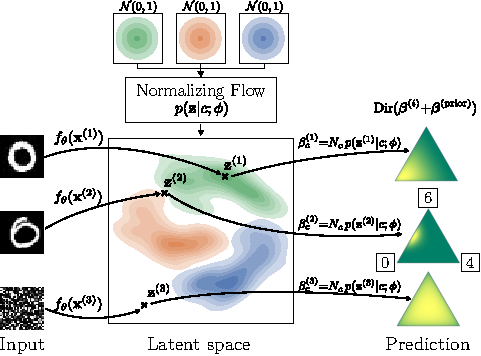
\includegraphics{sections/006_neurips2020/diagram/diagram_new-crop.pdf}
	}
	\caption{Overview of \PostNet.}
	\label{fig:overview}
	\vspace{-2cm}
\end{wrapfigure}

\paragraph{Overview.} In \cref{fig:overview} we provide an overview of \PostNet. We have three example inputs, \smash{$\vect{x}^{(1)}$,} \smash{$\vect{x}^{(2)}$}, and \smash{$\vect{x}^{(3)}$}, which are mapped onto their respective latent space coordinates $\latent\dataix$ by the encoding neural network $f_\theta$. The normalizing flow component learns flexible (normalized) density functions $\prob(\latent|c;\phi)$, for which we evaluate their densities at the positions of the latent vectors \smash{$\latent\dataix$}. These densities are used to parameterize a Dirichlet distribution for each data point, as seen on the right hand side. Higher densities correspond to higher confidence in the Dirichlet distributions -- we can observe that the out-of-distribution sample \smash{$\vect{x}^{(3)}$} is mapped to a point with (almost) no density, and hence its predicted Dirichlet distribution has very high epistemic uncertainty. On the other hand, \smash{$\vect{x}^{(2)}$} is an ambiguous example that could depict either the digit 0 or 6. This is reflected in its corresponding Dirichlet distribution, which has high aleatoric uncertainty (as the sample is ambiguous), but low epistemic uncertainty (since it is from the distribution of hand-drawn digits). The unambiguous sample \smash{$\vect{x}^{(1)}$} has low overall uncertainty.

Lastly, since both the encoder network $f_\theta$ and the normalizing flow parameterized by $\phi$ are fully differentiable, we can learn their parameters jointly in an end-to-end fashion. We do this via a novel loss  defined in \cref{sec:uncertainty_loss_006} which emerges from Bayesian learning principles \cite{PAC-bayesian_estimator} and is related to \UCEacro \cite{uceloss}.

\subsection{Density estimation for OOD detection}

Normalized densities, as used by \PostNetacro, are well suited to discriminate between ID data (with high likelihoood) and OOD data (with low likelihood). While it is also possible to learn a normalizing flow model on the input domain directly (e.g., \cite{maf, why-nf-fail-ood, grathwohl2018scalable}), this is very computationally demanding and might not be necessary for a discriminative model. Futhermore, density estimation is prone to the curse of dimensionality in high dimensional spaces \cite{typicality_OOD_generative, anomaly-detection}. For example, unsupervised deep generative models like \cite{glow} or \cite{pixel_cnn} have been shown to be unable to distinguish between ID and OOD samples in some situations when working on all features directly \cite{deep-generative, energy_based_classifier}. 

To circumvent these issues, \PostNetacro leverages two techniques. First, it uses the full class label information. Thus, \PostNetacro assigns a density per class and regularizes the epistemic uncertainty with the training class counts $N_\iclass$. Second, \PostNetacro performs density estimation on a low dimensional latent space describing relevant features for the classification task (\cref{fig:mnist_2D_latent_space}; \cref{fig:overview}).
Hence, \PostNetacro does not suffer from the curse of dimensionality and still enjoys the benefits of a properly normalized density function. Using the inductive bias of a discriminative task and low dimensional latent representations improved OOD detection in  \cite{why-nf-fail-ood} as well.
